% Document mode
\documentclass[doc,longtable]{apa6}
\usepackage{longtable}
\usepackage{lmodern}
\usepackage[T1]{fontenc}
\usepackage[utf8]{inputenc}
\usepackage[american]{babel}
\usepackage{csquotes}
\usepackage{microtype}
\usepackage{amsmath,amssymb}
\usepackage{graphicx}
\usepackage{booktabs}
\usepackage{caption}
\usepackage{subcaption}
\usepackage[unicode=true]{hyperref}

% Pandoc stuff
\UseMicrotypeSet[protrusion]{basicmath}
\let\tightlist\relax % empty pandoc tight list command
\urlstyle{same} % url non-monotype

% Hyperlinks and other metadata in pdf
\hypersetup{unicode=true,
            pdftitle={Writing an APA manuscript from Pandoc markdown},
            pdfauthor={Author 1, Author 2; Author 3},
            pdfkeywords={sublime text; vscode; pandoc; apa6},
            pdfborder={0 0 0},
            colorlinks=true,
            linkcolor=blue,
            citecolor=blue,
            urlcolor=blue,
            breaklinks=true}

% References
\usepackage[backend=biber,sortcites=true,style=apa,sorting=nyt,isbn=false,url=false]{biblatex}
\DeclareLanguageMapping{american}{american-apa}
\addbibresource{example/references.bib}

% Title page stuff
\title{Writing an APA manuscript from Pandoc markdown}
\shorttitle{APA from markdown}
\twoauthors{Author 1, Author 2}{Author 3}
\twoaffiliations{Institute 1}{Institute 2}

\note{Last updated: \today}
\authornote{%
\noindent Correspondence:

Joseph M. Burling

Department of Psychology

6538 Franz Hall, UCLA

Los Angeles, CA 90095-1563

Email: jmburling@ucla.edu
}

% Abstract page
\abstract{%
This is just an example of using pandoc (with the help of some build systems) to write in pandoc's markdown syntax for APA manuscripts. The output will be rendered in APA 6 format according to some commands and class options provided by the LaTeX \texttt{apa6} package. I also make use of a few pandoc filters downloaded as python modules to get cross-referencing to work. Lastly, I provide a .DOCX version of the build system, though a lot may not translate and will require some additional tweaking.
}

\keywords{sublime text, vscode, pandoc, apa6}

\begin{document}
\maketitle

% pandoc-xnos: macro to create a caption without a prefix
\makeatletter
\def\LT@makenoprefixcaption#1#2#3{%
  \LT@mcol\LT@cols c{\hbox to\z@{\hss\parbox[t]\LTcapwidth{
    \sbox\@tempboxa{#1{}#3}
    \ifdim\wd\@tempboxa>\hsize
      #1{}#3
    \else
      \hbox to\hsize{\hfil\box\@tempboxa\hfil}%
    \fi
    \endgraf\vskip\baselineskip}
  \hss}}}
\makeatother

% pandoc-tablenos: save original macros
\makeatletter
\let\LT@oldmakecaption=\LT@makecaption
\let\oldthetable=\thetable
\let\oldtheHtable=\theHtable
\makeatother

% pandoc-tablenos: environment disables table caption prefixes
\makeatletter
\newcounter{tableno}
\newenvironment{no-prefix-table-caption}{
  \let\LT@makecaption=\LT@makenoprefixcaption
  \renewcommand\thetable{x.\thetableno}
  \renewcommand\theHtable{x.\thetableno}
  \stepcounter{tableno}
}{
  \let\thetable=\oldthetable
  \let\theHtable=\oldtheHtable
  \let\LT@makecaption=\LT@oldmakecaption
  \addtocounter{table}{-1}
}
\makeatother

\section{Quick pandoc overview}\label{quick-pandoc-overview}

Words go here, also here is a citation \autocite{someArticle}. According to \textcite{anotherArticle}, something bad happened. See Figure \ref{fig:myplot}. This is a bold statement\ldots{} \textbf{WOW!}, and here's \_some \emph{emphasis for you} too. Sometimes you need some typewrite-like font, like when writing code: \texttt{my\_answer\ =\ 1\ +\ 1}. Other types you may need to write blocks of code, like this:

\begin{verbatim}
\begin{table}
\centering
\begin{tabular}{|l|l|}\hline
Age & Frequency \\ \hline
18--25  & 15 \\
26--35  & 33 \\
36--45  & 22 \\ \hline
\end{tabular}
\end{table}
\end{verbatim}

\begin{figure}
\centering
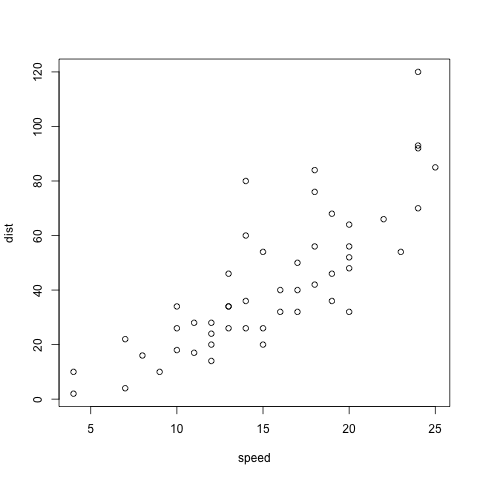
\includegraphics[width=3.00000in]{example/plot.png}
\caption{Your figure caption goes here.\label{fig:myplot}}
\end{figure}

See Table \ref{tbl:mytable} for an example on making tables using the default extension. In APA man mode, Tables are sent to the end of the document unless the following is used in the YAML header at the top of this document:

\begin{verbatim}
classoption:
    - floatsintext
\end{verbatim}

\begin{longtable}[]{@{}rllc@{}}
\caption{A table. \label{tbl:mytable}}\tabularnewline
\toprule
Right & Left & Default & Center\tabularnewline
\midrule
\endfirsthead
\toprule
Right & Left & Default & Center\tabularnewline
\midrule
\endhead
12 & 12 & 12 & 12\tabularnewline
123 & 123 & 123 & 123\tabularnewline
1 & 1 & 1 & 1\tabularnewline
\bottomrule
\end{longtable}

\begin{itemize}
\tightlist
\item
  This is another type of pandoc table (\ref{tbl:anotherone}). It should look the same.\footnote{Sometimes docx files will have tables that are squished. Autofit the document width to fix.}
\end{itemize}

\begin{longtable}[]{@{}rllc@{}}
\caption{Another one \label{tbl:anotherone}}\tabularnewline
\toprule
Right & Left & Default & Center\tabularnewline
\midrule
\endfirsthead
\toprule
Right & Left & Default & Center\tabularnewline
\midrule
\endhead
12 & 12 & 12 & 12\tabularnewline
123 & 123 & 123 & 123\tabularnewline
1 & 1 & 1 & 1\tabularnewline
\bottomrule
\end{longtable}

\newpage

\begin{no-prefix-table-caption}

\begin{longtable}[]{@{}lll@{}}
\caption{And another multi-line table which is more complicated to make. It may requires a pagebreak in two-column (jou) mode because pandoc uses \texttt{longtable} which doesn't work in two-column mode.Some additional latex hacks are added to the template to allow it to work (at the risk of losing content or bleeding off the page. Blame pandoc for using \texttt{longtable}).}\tabularnewline
\toprule
\begin{minipage}[b]{0.20\columnwidth}\raggedright\strut
Fruit\strut
\end{minipage} & \begin{minipage}[b]{0.20\columnwidth}\raggedright\strut
Price\strut
\end{minipage} & \begin{minipage}[b]{0.27\columnwidth}\raggedright\strut
Advantages\strut
\end{minipage}\tabularnewline
\midrule
\endfirsthead
\toprule
\begin{minipage}[b]{0.20\columnwidth}\raggedright\strut
Fruit\strut
\end{minipage} & \begin{minipage}[b]{0.20\columnwidth}\raggedright\strut
Price\strut
\end{minipage} & \begin{minipage}[b]{0.27\columnwidth}\raggedright\strut
Advantages\strut
\end{minipage}\tabularnewline
\midrule
\endhead
\begin{minipage}[t]{0.32\columnwidth}\raggedright\strut
Bananas\strut
\end{minipage} & \begin{minipage}[t]{0.32\columnwidth}\raggedright\strut
\$1.34\strut
\end{minipage} & \begin{minipage}[t]{0.32\columnwidth}\raggedright\strut
\begin{itemize}
\tightlist
\item
  built-in wrapper
\item
  bright color
\end{itemize}\strut
\end{minipage}\tabularnewline
\begin{minipage}[t]{0.32\columnwidth}\raggedright\strut
Oranges\strut
\end{minipage} & \begin{minipage}[t]{0.32\columnwidth}\raggedright\strut
\$2.10\strut
\end{minipage} & \begin{minipage}[t]{0.32\columnwidth}\raggedright\strut
\begin{itemize}
\tightlist
\item
  cures scurvy
\item
  tasty
\end{itemize}\strut
\end{minipage}\tabularnewline
\bottomrule
\end{longtable}

\end{no-prefix-table-caption}

\begin{itemize}
\tightlist
\item
  Here's some raw latex code. It won't be recognized unless the output is LaTeX/pdf and you have to proper parse-raw option set. It's the same LaTeX code block from above rendered as an actual Table \ref{tbl:rawtex}. The position may shift because it's a floating environment.
\end{itemize}

\begin{table}
\centering
\caption{Using raw latex code}
\label{tbl:rawtex}
\begin{tabular}{|l|l|}\hline
Age & Frequency \\ \hline
18--25  & 15 \\
26--35  & 33 \\
36--45  & 22 \\ \hline
\end{tabular}
\end{table}

\begin{itemize}
\item
  Here's an example of inline LaTeX math, \(p=.0499\).
\item
  Here's a an example of using LaTeX syntax for displaying equations.
\end{itemize}

\[
\hat{y} = \beta_0 + \beta_1 x
\]

Pandoc doesn't know how to make inline headings when converting to Word. If you put the cursor at the end of the heading, press Ctrl+Alt+Enter and it will move it down.

\subsection{Subsection heading}\label{subsection-heading}

Lorem ipsum dolor sit amet, consectetur adipiscing elit. Nulla et magna vitae ipsum rhoncus congue eu vehicula sem. Vestibulum venenatis mauris ac urna porta placerat. Ut ante neque, malesuada ut lobortis ullamcorper, consectetur vitae ipsum. Morbi sodales, justo eu pretium venenatis, sem libero dapibus sem, at molestie lectus felis ut nunc. Praesent ultrices sagittis porta. Curabitur diam elit, lacinia nec egestas sit amet, convallis a felis. Praesent dictum nec mauris quis molestie. Proin ullamcorper, mauris sed molestie aliquet, nisi sapien tempor risus, quis congue sapien turpis et justo. Suspendisse potenti.

Duis viverra aliquet metus, eget aliquam tellus mollis imperdiet. Lorem ipsum dolor sit amet, consectetur adipiscing elit. Nulla et magna vitae ipsum rhoncus congue eu vehicula sem. Vestibulum venenatis mauris ac urna porta placerat. Ut ante neque, malesuada ut lobortis ullamcorper, consectetur vitae ipsum. Morbi sodales, justo eu pretium venenatis, sem libero dapibus sem, at molestie lectus felis ut nunc. Praesent ultrices sagittis porta. Curabitur diam elit, lacinia nec egestas sit amet, convallis a felis.

\subsubsection{Subsubsection heading}\label{subsubsection-heading}

Nullam nec est ut mauris eleifend pulvinar ac in nisl. In eleifend, velit et rhoncus pretium, justo lectus viverra enim, nec feugiat ante mauris vitae magna. Lorem ipsum dolor sit amet, consectetur adipiscing elit. Morbi felis nulla, iaculis dapibus sapien quis, pretium laoreet est. Mauris vel sapien tempor, dapibus ipsum sit amet, sagittis tellus. Aliquam ipsum metus, ultricies eleifend dolor nec, ultricies mollis sapien. Integer placerat ante condimentum sagittis elementum. Fusce aliquam, libero a iaculis eleifend, ipsum ante tincidunt ante, ut bibendum dolor risus ut nibh. Sed fermentum tellus id ligula sodales, ut condimentum tortor tempus. Phasellus suscipit dapibus est sed consectetur.

Nullam nec est ut mauris eleifend pulvinar ac in nisl. In eleifend, velit et rhoncus pretium, justo lectus viverra enim, nec feugiat ante mauris vitae magna. Lorem ipsum dolor sit amet, consectetur adipiscing elit. Morbi felis nulla, iaculis dapibus sapien quis, pretium laoreet est. Mauris vel sapien tempor, dapibus ipsum sit amet, sagittis tellus. Aliquam ipsum metus, ultricies eleifend dolor nec, ultricies mollis sapien. Integer placerat ante condimentum sagittis elementum. Fusce aliquam, libero a iaculis eleifend, ipsum ante tincidunt ante, ut bibendum dolor risus ut nibh. Sed fermentum tellus id ligula sodales, ut condimentum tortor tempus. Phasellus suscipit dapibus est sed consectetur.

\paragraph{Paragraph heading}\label{paragraph-heading}

Lorem ipsum dolor sit amet, consectetur adipiscing elit. Nulla et magna vitae ipsum rhoncus congue eu vehicula sem. Vestibulum venenatis mauris ac urna porta placerat. Ut ante neque, malesuada ut lobortis ullamcorper, consectetur vitae ipsum. Morbi sodales, justo eu pretium venenatis, sem libero dapibus sem, at molestie lectus felis ut nunc. Praesent ultrices sagittis porta. Curabitur diam elit, lacinia nec egestas sit amet, convallis a felis. Praesent dictum nec mauris quis molestie. Proin ullamcorper, mauris sed molestie aliquet, nisi sapien tempor risus, quis congue sapien turpis et justo. Suspendisse potenti. Duis viverra aliquet metus, eget aliquam tellus mollis imperdiet.

\subparagraph{Subparagraph heading}\label{subparagraph-heading}

Lorem ipsum dolor sit amet, consectetur adipiscing elit. Nulla et magna vitae ipsum rhoncus congue eu vehicula sem. Vestibulum venenatis mauris ac urna porta placerat. Ut ante neque, malesuada ut lobortis ullamcorper, consectetur vitae ipsum. Morbi sodales, justo eu pretium venenatis, sem libero dapibus sem, at molestie lectus felis ut nunc. Praesent ultrices sagittis porta. Curabitur diam elit, lacinia nec egestas sit amet, convallis a felis. Praesent dictum nec mauris quis molestie. Proin ullamcorper, mauris sed molestie aliquet, nisi sapien tempor risus, quis congue sapien turpis et justo. Suspendisse potenti. Duis viverra aliquet metus, eget aliquam tellus mollis imperdiet.

Getting silly with the amount of subheadings

Lorem ipsum dolor sit amet, consectetur adipiscing elit. Nulla et magna vitae ipsum rhoncus congue eu vehicula sem. Vestibulum venenatis mauris ac urna porta placerat. Ut ante neque, malesuada ut lobortis ullamcorper, consectetur vitae ipsum. Morbi sodales, justo eu pretium venenatis, sem libero dapibus sem, at molestie lectus felis ut nunc. Praesent ultrices sagittis porta. Curabitur diam elit, lacinia nec egestas sit amet, convallis a felis. Praesent dictum nec mauris quis molestie. Proin ullamcorper, mauris sed molestie aliquet, nisi sapien tempor risus, quis congue sapien turpis et justo. Suspendisse potenti. Duis viverra aliquet metus, eget aliquam tellus mollis imperdiet.

Nullam nec est ut mauris eleifend pulvinar ac in nisl. In eleifend, velit et rhoncus pretium, justo lectus viverra enim, nec feugiat ante mauris vitae magna. Lorem ipsum dolor sit amet, consectetur adipiscing elit. Morbi felis nulla, iaculis dapibus sapien quis, pretium laoreet est. Mauris vel sapien tempor, dapibus ipsum sit amet, sagittis tellus. Aliquam ipsum metus, ultricies eleifend dolor nec, ultricies mollis sapien. Integer placerat ante condimentum sagittis elementum. Fusce aliquam, libero a iaculis eleifend, ipsum ante tincidunt ante, ut bibendum dolor risus ut nibh. Sed fermentum tellus id ligula sodales, ut condimentum tortor tempus. Phasellus suscipit dapibus est sed consectetur.

\newpage

\printbibliography[title=References]


\end{document}
